\documentclass[border=5mm]{standalone}
\usepackage{pgfplots}
\usepackage{amssymb, amsmath}
\usetikzlibrary{decorations, arrows.meta}
\pgfplotsset{compat=newest}

\makeatletter
        \pgfdeclareplotmark{dot}
        {
            \fill circle [x radius=0.02, y radius=0.08];
        }
\makeatother

\begin{document}
% credit goes to:
% https://tex.stackexchange.com/questions/254484/how-to-make-a-graph-of-heteroskedasticity-with-tikz-pgf 
% for much of the original code and inspiration 

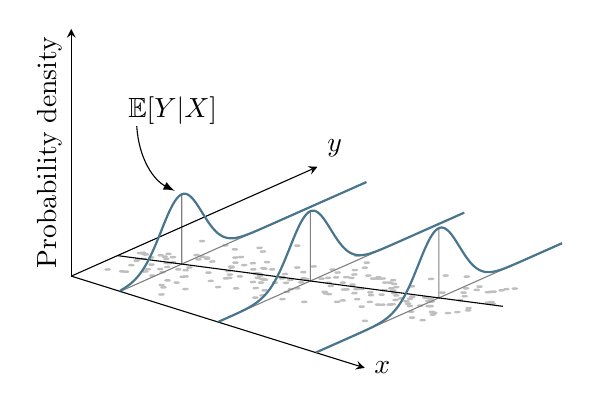
\begin{tikzpicture}[ % Define Normal Probability Function
declare function={
            normal(\x,\m,\s) = 1/(2*\s*sqrt(pi))*exp(-(\x-\m)^2/(2*\s^2));
        },
    declare function={invgauss(\a,\b) = sqrt(-2*ln(\a))*cos(deg(2*pi*\b));}
       ]
\begin{axis}[
    domain=0:12,
    zmin=0, zmax=1,
    xmin=0, xmax=3,
    samples=200,
   samples y=0,
    view={40}{30},
    axis lines=middle,
    enlarge y limits=false,
    xtick=\empty,
    xmajorgrids,
    xticklabels={},
    ytick=\empty,
    xticklabels=\empty,
    ztick=\empty,
    xlabel=$x$, xlabel style={at={(rel axis cs:1,0,0)}, anchor=west},
    ylabel=$y$, ylabel style={at={(rel axis cs:0,1,0)}, anchor=south west},
    zlabel=Probability density, zlabel style={at={(rel axis cs:0,0,0.5)}, rotate=90, anchor=south},
    set layers, mark=cube
  ]


\draw [-latex, shorten >= 1mm]  (0.25, 2, {normal(0,0,.5)}) to [bend right] (.5, 3, {normal(0,0,1)});
\node at (0.25, 3.75, {normal(0,0,.5)}) {$\mathbb E[Y|X]$};

\addplot3 [gray!50, only marks, mark=dot, mark layer=like plot, samples=200, domain=0.1:2.9, on layer=axis background] (x, {1.5*(x-0.5)+3+invgauss(rnd,rnd)}, 0);
\addplot3 [samples=2, samples y=0, domain=0:3] (x, {1.5*(x-0.5)+3}, 0);
\addplot3 [cyan!50!black, thick] (0.5, x, {normal(x, 3, 1)});
\addplot3 [cyan!50!black, thick] (1.5, x, {normal(x, 4.5, 1)});
\addplot3 [cyan!50!black, thick] (2.5, x, {normal(x, 6, 1)});


\pgfplotsextra{
\begin{pgfonlayer}{axis background}

\draw [gray, on layer=axis background] (0.5, 3, 0) -- (0.5, 3, {normal(0,0,1)}) (0.5,0,0) -- (0.5,12,0)
    (1.5, 4.5, 0) -- (1.5, 4.5, {normal(0,0,1)}) (1.5,0,0) -- (1.5,12,0)
    (2.5, 6, 0) -- (2.5, 6, {normal(0,0,1)}) (2.5,0,0) -- (2.5,12,0);

\end{pgfonlayer}
}


\end{axis}


\end{tikzpicture}

\end{document}
